\begin{question}
\noindent A space exploration museum displays a scale model of a rover on a grid map of an exhibition floor. Shape $R$ shows the rover's starting position. The rover is moved along the floor by the translation $\begin{pmatrix} 3 \\ -4 \end{pmatrix}$ to its new display position, shape $R'$.

\begin{center}
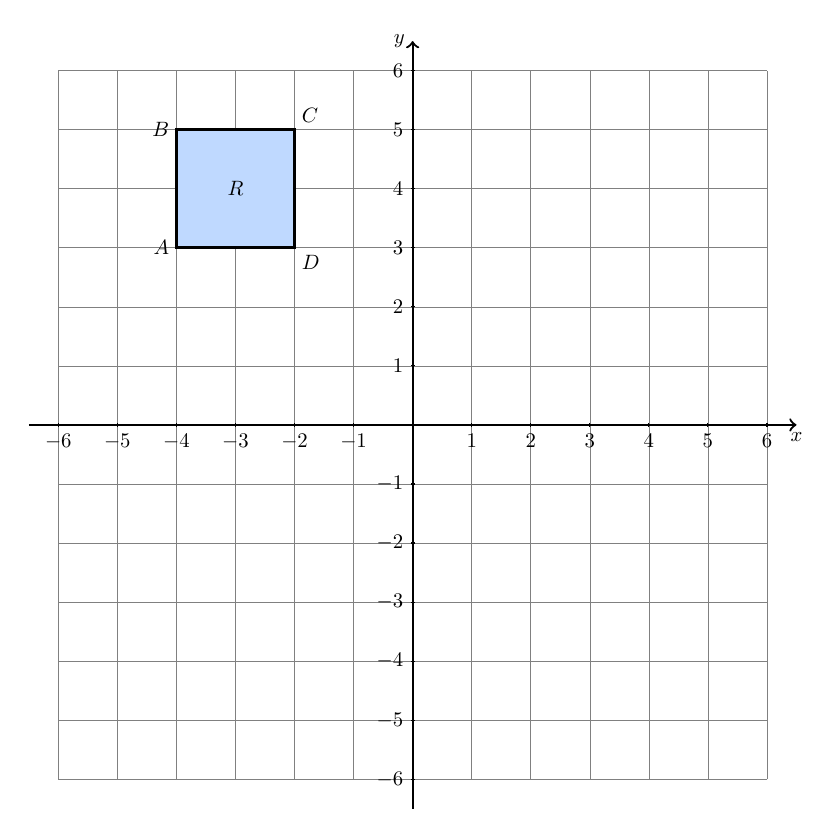
\begin{tikzpicture}[scale=0.75, transform shape]
    \def\axisLimit{6}

    \definecolor{borderColour}{HTML}{000000}
    \definecolor{fillColourR}{HTML}{BFD9FF}

    % Draw grid
    \draw[step=1cm,gray,very thin] (-\axisLimit,-\axisLimit) grid (\axisLimit,\axisLimit);

    % Draw axes
    \draw[thick,->] (-\axisLimit-0.5,0) -- (\axisLimit+0.5,0) node[anchor=north] {$x$};
    \draw[thick,->] (0,-\axisLimit-0.5) -- (0,\axisLimit+0.5) node[anchor=east] {$y$};

    % Label x-axis and y-axis
    \foreach \x in {-\axisLimit,...,-1,1,2,...,\axisLimit}
        \draw (\x cm,1pt) -- (\x cm,-1pt) node[anchor=north] {$\x$};
    \foreach \y in {-\axisLimit,...,-1,1,2,...,\axisLimit}
        \draw (1pt,\y cm) -- (-1pt,\y cm) node[anchor=east] {$\y$};

    % Shape R: vertices A(-4,3), B(-4,5), C(-2,5), D(-2,3)
    \coordinate (A) at (-4,3);
    \coordinate (B) at (-4,5);
    \coordinate (C) at (-2,5);
    \coordinate (D) at (-2,3);
    \filldraw[fill=fillColourR, draw=borderColour, line width=1pt] (A) -- (B) -- (C) -- (D) -- cycle;

    \node[left] at (A) {$A$};
    \node[left] at (B) {$B$};
    \node[above right] at (C) {$C$};
    \node[below right] at (D) {$D$};
    \node at (-3,4) {$R$};

\end{tikzpicture}
\end{center}

\noindent On the grid, draw the image of shape $R$ after a translation by the vector $\begin{pmatrix} 3 \\ -4 \end{pmatrix}$.\\
Label the image $R'$.

\vspace{4cm}

\begin{flushright}
    \answerplain{2}
\end{flushright}
\end{question}